\documentclass[border=0pt]{standalone}
\usepackage{tikz,amssymb,url,amsmath,amsthm,listings,algorithm,algpseudocode,enumerate, caption, xspace, float, verbatim,tabularx,mathtools,adjustbox,pgfplots}
\usetikzlibrary{fit}
\usetikzlibrary{positioning}
\usetikzlibrary{math}
\usetikzlibrary{shapes.misc}
\usetikzlibrary{backgrounds}
\def\bw{{\boldsymbol w}}
\def\bx{{\boldsymbol x}}
\def\balpha{{\boldsymbol \alpha}}
\pgfdeclarelayer{background}
\pgfsetlayers{background,main}
\tikzset{cross/.style={cross out, draw=black, minimum size=2*(#1-\pgflinewidth), inner sep=0pt, outer sep=0pt},cross/.default={1pt}}
\begin{document}
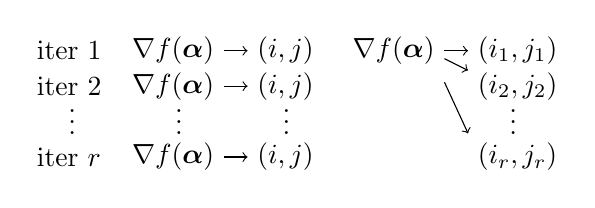
\begin{tikzpicture}[yscale=1,xscale=1,baseline,tight background]
	\tikzmath{\dx=2.5; \dy=-0.45; \darrow=0.3;
	\iax=0; \iay=0;
	\ibx=\iax; \iby=\iay+\dy;
	\icx=\iax; \icy=\iby+\dy;
	\idx=\iax; \idy=\icy+\dy;
	\gdax=\iax+\dx; \gday=\iay;
	\gdbx=\gdax; \gdby=\gday+\dy;
	\gdcx=\gdax; \gdcy=\gdby+\dy;
	\gddx=\gdax; \gddy=\gdcy+\dy;
	\gdijax=\gdax+\darrow; \gdijay=\gday;
	\gdijbx=\gdijax; \gdijby=\gdijay+\dy;
	\gdijcx=\gdijax; \gdijcy=\gdijby+\dy;
	\gdijdx=\gdijax; \gdijdy=\gdijcy+\dy;
	\smax=\gdijax+\dx; \smay=\gdijay;
	\smbx=\smax; \smby=\smay+\dy;
	\smcx=\smax; \smcy=\smby+\dy;
	\smdx=\smax; \smdy=\smcy+\dy;
	\smijax=\smax+\darrow; \smijay=\smay;
	\smijbx=\smijax; \smijby=\smijay+\dy;
	\smijcx=\smijax; \smijcy=\smijby+\dy;
	\smijdx=\smijax; \smijdy=\smijcy+\dy;
	\headax=\gdax; \headay=\gday-\dy;
	\headbx=\smax; \headby=\smay-\dy;
	}
	\node at (\iax,\iay)[right]{iter 1};
	\node at (\ibx,\iby)[right]{iter 2};
	\node at (\icx+0.4,\icy+0.1)[right]{$\vdots$};
	\node at (\idx,\idy)[right]{iter $r$};
	\node at (\gdax,\gday)[left]{$\nabla f(\balpha)$};
	\node at (\gdbx,\gdby)[left]{$\nabla f(\balpha)$};
	\node at (\gdcx-0.4,\gdcy+0.1)[left]{$\vdots$};
	\node at (\gddx,\gddy)[left]{$\nabla f(\balpha)$};
	\node at (\gdijax,\gdijay)[right]{$(i,j)$};
	\node at (\gdijbx,\gdijby)[right]{$(i,j)$};
	\node at (\gdijcx+0.32,\gdijcy+0.1)[right]{$\vdots$};
	\node at (\gdijdx,\gdijdy)[right]{$(i,j)$};
	\node at (\smax,\smay)[left]{$\nabla f(\balpha)$};
	\node at (\smbx,\smby)[left]{};
	\node at (\smcx+0.4,\smcy)[left]{};
	\node at (\smdx,\smdy)[left]{};
	\node at (\smijax,\smijay)[right]{$(i_1,j_1)$};
	\node at (\smijbx,\smijby)[right]{$(i_2,j_2)$};
	\node at (\smijcx+0.4,\smijcy+0.1)[right]{$\vdots$};
	\node at (\smijdx,\smijdy)[right]{$(i_r,j_r)$};
	%\node at (\headax,\headay)[]{Greedy Selection};
	%\node at (\headbx+0.2,\headby)[]{Second Approach};
	\draw[->] (\gdax,\gday) -- (\gdijax, \gdijay);
	\draw[->] (\gdbx,\gdby) -- (\gdijbx, \gdijby);
	\draw[->] (\gddx,\gddy) -- (\gdijdx, \gdijdy);
	\draw[->] (\smax,\smay) -- (\smijax, \smijay);
	\draw[->] (\smax,\smay-0.1) -- (\smijbx, \smijby+0.2);
	\draw[->] (\smax,\smay-0.4) -- (\smijdx, \smijdy+0.3);
\end{tikzpicture}
\end{document}
